\documentclass[aspectratio=169]{beamer}
\usetheme{Madrid}
\usecolortheme{seahorse}
\setbeamertemplate{navigation symbols}{}
\setbeamertemplate{footline}[frame number]

\usepackage[utf8]{inputenc}
\usepackage[T1]{fontenc}
\usepackage{lmodern}
\usepackage{graphicx}
\usepackage{amsmath,amssymb,mathtools}
\usepackage{hyperref}
\usepackage{xcolor}
\usepackage{listings}
% Simple diagram support
\usepackage{tikz}
\usetikzlibrary{arrows.meta,positioning}

\newcommand{\PA}[1]{{\textcolor{cyan}{[{\bfseries PA:} #1]}}}
\newcommand{\DeJ}[1]{{\textcolor{magenta}{[{\bfseries DJ:} #1]}}} % DJ was taken!
\newcommand{\AJ}[1]{{\textcolor{green}{[{\bfseries AJ:} #1]}}}
\newcommand{\GG}[1]{{\textcolor{blue}{[{\bfseries GG:} #1]}}}

% Map common Unicode symbols to LaTeX math (outside listings)
\usepackage{newunicodechar}
\newunicodechar{·}{\ensuremath{\cdot}}
\newunicodechar{⊙}{\ensuremath{\odot}}
\newunicodechar{ᵀ}{\ensuremath{^{\top}}}
\newunicodechar{×}{\ensuremath{\times}}
\newunicodechar{–}{-}
\newunicodechar{—}{-}

% Listing styles (Unicode-safe for later use)
\definecolor{terminalback}{rgb}{0.9,0.9,0.9}
\definecolor{terminaltext}{rgb}{0.1,0.1,0.1}
\lstdefinestyle{terminal}{
    backgroundcolor=\color{gray!20},
    basicstyle=\ttfamily\small\color{terminaltext},
    frame=single, rulecolor=\color{white}, breaklines=true,
    captionpos=b, showstringspaces=false,
    upquote=true, columns=fullflexible,
    commentstyle=\color{terminaltext},
    keywordstyle=\color{terminaltext},
    stringstyle=\color{terminaltext},
    identifierstyle=\color{terminaltext},
    literate={·}{{$\cdot$}}1 {⊙}{{$\odot$}}1 {ᵀ}{{$^\top$}}1 {×}{{$\times$}}1 {‐}{{-}}1 {–}{{-}}1 {—}{{-}}1
}
\lstdefinestyle{code}{
    backgroundcolor=\color[rgb]{0.95,0.95,0.95},
    basicstyle=\ttfamily\small, frame=single, breaklines=true, showstringspaces=false,
    rulecolor=\color{black}, numbers=none, keepspaces=true, captionpos=b, tabsize=2,
    language=C++,
    literate={·}{{$\cdot$}}1 {⊙}{{$\odot$}}1 {ᵀ}{{$^\top$}}1 {×}{{$\times$}}1 {‐}{{-}}1 {“}{{"`}}1 {”}{{'"}}1
}


\lstdefinestyle{cpp-rich}{
  language=C++,
  basicstyle=\ttfamily\scriptsize,
  keywordstyle=\color{blue}\bfseries,
  identifierstyle=\color{black},
  commentstyle=\color{gray}\itshape,
  stringstyle=\color{green!50!black},
  morekeywords={nullptr,override,final,constexpr},
  showstringspaces=false,
  upquote=true,
  frame=single,
  rulecolor=\color{black},
  breaklines=true,
  columns=fullflexible,
  keepspaces=true,
  tabsize=2,
  backgroundcolor=\color[rgb]{0.95,0.95,0.95},
  literate={·}{{$\cdot$}}1 {⊙}{{$\odot$}}1 {ᵀ}{{$^\top$}}1 {×}{{$\times$}}1 {‐}{{-}}1 {–}{{-}}1 {—}{{-}}1 {“}{{"`}}1 {”}{{'"}}1
}
% make it the default
\lstset{style=cpp-rich}
% alias macro (use in optional args: \begin{lstlisting}[\cpplistingstyle])
\newcommand{\cpplistingstyle}{style=cpp-rich}

\title{Algebraic Programming (ALP) Tutorial}
%\subtitle{From HPC to GraphBLAS and Transition Paths}
\author{ALP HIPO Team}
\date{\today}

% Show roadmap before each section/subsection with upcoming content highlighted
\AtBeginSection{
  \begin{frame}{Roadmap}
    \tableofcontents[currentsection,sectionstyle=show/shaded,subsectionstyle=show/show/hide]
  \end{frame}
}
\AtBeginSubsection{
  \begin{frame}{Roadmap}
    \tableofcontents[currentsection,currentsubsection,sectionstyle=show/shaded,subsectionstyle=show/shaded/hide]
  \end{frame}
}

\begin{document}
\frame{\titlepage}

% =========================
% Monday 10 Nov, Morning
% =========================
\section{Monday 10 Nov, Morning}

% One initial agenda slide for Monday; will be auto-repeated via Roadmap frames
\begin{frame}{Today's Plan}
Morning:
\begin{enumerate}
  \item Introduction to ALP, installation, and short demos
  \item Hands-on (I): installation, containers, I/O, copying, masking, and standard matrices
  \item Introduction to core primitives
  \item Hands-on (II): numerical linear algebra
  \item Interoperability with existing code: transition paths \& Python
\end{enumerate}\vspace{\baselineskip}

Afternoon:
\begin{enumerate}\setcounter{enumi}{6}
	\item Ising Machine, and
	\item other solvers
\end{enumerate}
\end{frame}

\subsection{1) Introduction to ALP, installation, and short demos}
% Owner: DJ

% Intro (concise outline)
\begin{frame}{Introduction to GraphBLAS and ALP}
\begin{itemize}
  \item What you'll learn: algebraic programming for graphs and sparse data
  \item Who it's for: HPC developers and solver authors
  \item How we'll use ALP: C++ headers, precompiled libraries, Python API
\end{itemize}
% Owner: DJ
% TODO: add a one-slide agenda summary graphic
\end{frame}

% Slide 1
\begin{frame}{Goals, Audience, and Scope}
\begin{itemize}
  \item Goals
    \begin{itemize}
      \item Express algorithms as algebra over vectors/matrices
      \item Introduce GraphBLAS: containers, semirings, primitives, masks
      \item Demonstrate ALP backends for performance portability
    \end{itemize}
  \item Audience
    \begin{itemize}
      \item Developers of HPC applications, graph analytics, and solvers
      \item No prior GraphBLAS/ALP knowledge assumed
    \end{itemize}
  \item Scope: multiple usage modes
    \begin{itemize}
      \item C++ header library for new algorithms/solvers (template API)
      \item Precompiled libraries: use provided algorithms as black boxes
      \item Python API for precompiled algorithms
    \end{itemize}
\end{itemize}
% Owner: DJ
% Source: ALP_Tutorial.tex (intro), alp_graphblas_tutorial.txt (overview)
\end{frame}

% Slide 2
\begin{frame}{ALP in One Slide: Programming Model and Backends}
\begin{itemize}
  \item Programming model (humble by design)
    \begin{itemize}
      \item Heavily templated C++ header library (no runtime codegen)
      \item Hardware-unaware, hardware-independent user code
      \item Algebraic API: write what to compute, not how
    \end{itemize}
  \item Backends handle hardware specifics
    \begin{itemize}
      \item reference (single-threaded), \texttt{reference\_omp} (OpenMP)
      \item nonblocking (multi-threaded with auto-fusion)
      \item bsp1d (distributed/LPF), dense-dispatch (BLAS-backed, WIP), tensor (experimental, WIP)
      \item Same source runs across backends with consistent semantics
    \end{itemize}
  \item Flexible infrastructure
    \begin{itemize}
      \item Rich type system and traits enable different and mixed data-type operations
      \item Compile-time algebraic properties (associative, commutative, idempotent, annihilators)
            are known to the backends and propagate from top to bottom of the algorithm
    \end{itemize}
\end{itemize}

% Owner: DJ
\end{frame}

% Slide 2b (graphic)
\begin{frame}{ALP in One Slide: Programming Model and Backends (Graphic)}
\centering
\scriptsize
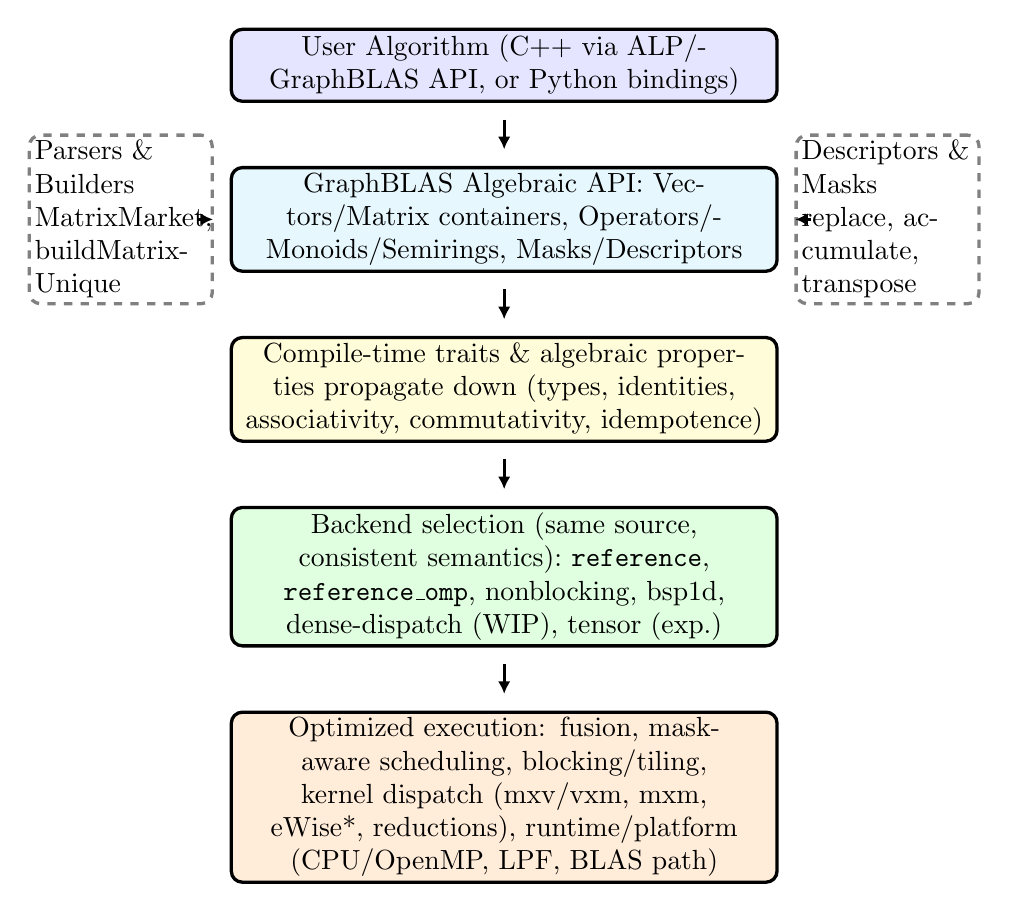
\begin{tikzpicture}[
  node distance=8mm and 6mm,
  mainbox/.style={rounded corners, draw, very thick, align=center, inner sep=2pt, minimum height=0.75cm, text width=.56\linewidth},
  sidebox/.style={rounded corners, draw, very thick, align=left, inner sep=2pt, text width=.18\linewidth},
  arrow/.style={-{Latex[length=1.6mm,width=1.6mm]}, very thick, shorten >=6pt, shorten <=6pt}
]
  % Main vertical flow (compact stack)
  \node[mainbox, fill=blue!10] (user) {User Algorithm (C++ via ALP/GraphBLAS API, or Python bindings)};
  \node[mainbox, fill=cyan!10, below=8mm of user] (api) {GraphBLAS Algebraic API: Vectors/Matrix containers, Operators/Monoids/Semirings, Masks/Descriptors};
  % Compile-time traits note placed between API and Backends
  \node[mainbox, fill=yellow!15, below=8mm of api] (traits) {Compile-time traits \& algebraic properties propagate down (types, identities, associativity, commutativity, idempotence)};
  \node[mainbox, fill=green!12, below=8mm of traits] (backends) {Backend selection (same source, consistent semantics):\ \texttt{reference}, \texttt{reference\_omp}, nonblocking, bsp1d, dense-dispatch (WIP), tensor (exp.)};
  \node[mainbox, fill=orange!15, below=8mm of backends] (exec) {Optimized execution: fusion, mask-aware scheduling, blocking/tiling, kernel dispatch (mxv/vxm, mxm, eWise*, reductions), runtime/platform (CPU/OpenMP, LPF, BLAS path)};

  \draw[arrow] (user) -- (api);
  \draw[arrow] (backends) -- (exec);

  % Side inputs/metadata
  \node[sidebox, dashed, draw=gray, fill=white, right=2mm of api] (desc) {Descriptors \& Masks\\ replace, accumulate, transpose};
  \draw[arrow, dashed] (desc.west) -- (api.east);

  \node[sidebox, dashed, draw=gray, fill=white, left=2mm of api] (io) {Parsers \& Builders\\ MatrixMarket, buildMatrixUnique};
  \draw[arrow, dashed] (io.east) -- (api.west);

  \draw[arrow] (api.south) -- (traits.north);
  \draw[arrow] (traits.south) -- (backends.north);
\end{tikzpicture}
\end{frame}

% Slide 3
\begin{frame}{What is GraphBLAS: Concepts and Motivation}
\begin{itemize}
  \item Motivation
    \begin{itemize}
      \item Graphs map to sparse matrices; algorithms to linear algebra
      \item Sparse/graph workloads are bandwidth-bound and irregular
    \end{itemize}
  \item Core concepts
    \begin{itemize}
      \item Semirings $\langle D,\oplus,\otimes\rangle$ (plus–times, min–plus, Boolean)
      \item Primitives: mxv/vxm, mxm, eWiseAdd/Mul/Apply, dot, masks, descriptors
      \item Containers: \texttt{grb::Vector<T>}, \texttt{grb::Matrix<T>}
    \end{itemize}
  \item Why beyond traditional dense LA
    \begin{itemize}
      \item Algebraic flexibility enables BFS, SSSP, etc., via non-standard "addition" and "multiplication"
      \item Masking and sparsity-aware execution preserve efficiency
    \end{itemize}
\end{itemize}
% Owner: DJ
% Source: alp_graphblas_tutorial.txt (GraphBLAS), ALP_Tutorial.tex (ALP/GraphBLAS)
\end{frame}

% Slide 4
\begin{frame}{Automation and Optimization Space}
\begin{itemize}
  \item What automation to expect (from ALP backends)
    \begin{itemize}
      \item Auto-parallel execution (threads/processes) across backends
      \item Cache-aware blocking/tiling; minimized data movement
      \item Mask-aware computation and potential kernel fusion (backend-dependent)
    \end{itemize}
  \item Algorithm-level optimization space (ALP vs. BLAS/LAPACK)
    \begin{itemize}
      \item ALP: end-to-end algebraic programs expose global opportunities
            (fusion across primitives, mask-driven sparsity cuts, reordering, schedule selection)
      \item LAPACK: dense factorizations focus on tiling and blocking inside fixed algorithms
      \item BLAS-only: kernel-local tuning; limited visibility for cross-kernel optimizations
    \end{itemize}
  \item Portability outcome
    \begin{itemize}
      \item Express once at the algebraic level; get optimized code on shared, distributed, or hybrid memory systems
      \item Mixed-type and custom-operator workflows supported via templates
    \end{itemize}
\end{itemize}
% Owner: DJ
% TODO: add a tiny mxv code snippet + "same code, different backend" example timings
% Source: ALP_Tutorial.tex (semantics, portability), alp_graphblas_tutorial.txt (landscape)
\end{frame}

% (Duplicate intro frames removed below to avoid repetition)


\begin{frame}[fragile]{1. ALP Installation}
\framesubtitle{Prerequisites (skip if already installed)}
\begin{itemize}
    \item Requirements:
    \begin{itemize}
        \item C++11 compiler, OpenMP, CMake (>=3.13), libNUMA, pthreads
    \end{itemize}
    \item Debian/Ubuntu:
\begin{lstlisting}[style=terminal, language=bash]
sudo apt-get install build-essential libnuma-dev libpthread-stubs0-dev cmake
\end{lstlisting}
    \item Red Hat/CentOS:
\begin{lstlisting}[style=terminal, language=bash]
dnf group install "Development Tools"
dnf install numactl-devel cmake
\end{lstlisting}
    \item Clone \textbf{ALP-Tutorial} from the official GitHub repository:
\begin{lstlisting}[style=terminal, language=bash]
git clone https://github.com/Algebraic-Programming/ALP-Tutorial.git
\end{lstlisting}
\end{itemize}
% Owner: PA
% Source (ALP_Tutorial.tex - Installation on Linux, step 1)
\end{frame}

\begin{frame}[fragile]{1. ALP Installation}
\framesubtitle{Obtain and Build ALP}
\begin{enumerate}
    \item Clone \textbf{ALP} from the official GitHub repository:
\begin{lstlisting}[style=terminal, language=bash]
git clone https://github.com/Algebraic-Programming/ALP.git
\end{lstlisting}
    \item Build and install \textbf{ALP} with default configuration settings:
\begin{lstlisting}[style=terminal, language=bash]
cd ALP && mkdir build && cd build
../bootstrap.sh --prefix=../install
make -j
make install
\end{lstlisting}
    \item \textbf{Activate ALP environment}:
\begin{lstlisting}[style=terminal, language=bash]
source ../install/bin/setenv
\end{lstlisting}
\end{enumerate}
% Owner: PA
% Source (ALP_Tutorial.tex - Installation on Linux, steps 2-3)
\end{frame}

\begin{frame}[fragile]{1. ALP Installation}
\framesubtitle{Setup Environment and Test}
\begin{enumerate}
    \item Return to the \textbf{ALP-Tutorial} directory:
\begin{lstlisting}[style=terminal, language=bash]
cd ../ALP-Tutorial/scripts
\end{lstlisting}
    \item \textbf{Compile example}:
\begin{lstlisting}[style=terminal, language=bash]
grbcxx sp.cpp -o sp_example
\end{lstlisting}
    \item \textbf{Run}:
\begin{lstlisting}[style=terminal, language=bash]
grbrun ./sp_example
\end{lstlisting}
\end{enumerate}
% Owner: PA
% Source (ALP_Tutorial.tex - Installation on Linux, steps 4-6)
\end{frame}

\begin{frame}[fragile]{2. Hands-on: Setting up scripts}
    \framesubtitle{ALP/GraphBLAS Overview}
    \begin{itemize}
        \item You can find code skeletons for the tutorial in: \texttt{path/to/alp-tutorial/scripts}
%         \item You should copy the scripts to your home directory: 
% \begin{lstlisting}[style=terminal, language=bash]
% cp -r /some/path/to/alp/tutorial/scripts ~/alp_tutorial_scripts
% cd ~/alp_tutorial_scripts && ls -l
%\end{lstlisting}
        \item You can use any editor of your preference to edit these scripts (e.g. nano, vim, gedit)
        \item Run these commands to test your setup:
\begin{lstlisting}[style=terminal, language=bash]
grbcxx alp_hw.cpp
grbrun ./a.out
\end{lstlisting}
\item \textbf{Expected output}:
\begin{lstlisting}[style=terminal, language=bash]
Info: grb::init (reference) called.
Hello from ./a.out
Info: grb::finalize (reference) called.
\end{lstlisting}
    \end{itemize}
\end{frame}

\begin{frame}[fragile]{2. Hands-on: What did we just run?}
    \framesubtitle{Hello World in ALP/GraphBLAS}
    \vspace{-0.6em}
    \begin{lstlisting}[style=cpp-rich, language=C++, basicstyle=\ttfamily\scriptsize]
#include <cstddef>
#include <cstring>
#include <graphblas.hpp>
#include <assert.h>

constexpr size_t max_fn_size = 255;
typedef char Filename[ max_fn_size ];

void hello_world( const Filename &in, int &out ) {
    std::cout << "Hello from " << in << std::endl;
    out = 0;
}

int main( int argc, char ** argv ) {
    Filename fn;
    std::strncpy( fn, argv[0], max_fn_size );
    int error_code = 100;
    
    grb::Launcher< grb::AUTOMATIC > launcher;
    assert( launcher.exec( &hello_world, fn, error_code, true ) == grb::SUCCESS );
    return error_code;
}
        \end{lstlisting}
        % Owner: PA
        % Source (ALP_Tutorial.tex - ALP/GraphBLAS, Hello World)
\end{frame}

\begin{frame}{2. Hands-on: What did we just run?}
\framesubtitle{ALP/GraphBLAS Overview}
\begin{itemize}
    \item Pure C++ (developed similarly to the GraphBLAS C specification)
    \item Exposes a GraphBLAS interface with 3 categories (part of the \texttt{grb} namespace):
    \begin{itemize}
        \item Algebraic containers (vectors, matrices, etc.)
        \item Algebraic structures (binary operators, semirings, etc.)
        \item Algebraic operations (take containers and structures as arguments)
    \end{itemize}
    \item \textbf{\texttt{grb::Launcher}}:
    \begin{itemize}
        \item Wraps calls to ALP programs
        \item Adapts to run-time conditions (e.g., distributed execution)
        \item \textbf{Question:} Why is the last argument to \texttt{launcher.exec} \texttt{true}?
        \begin{itemize}
            \item Consider the programmer reference documentation for the \texttt{grb::Launcher}...
        \end{itemize}
    \end{itemize}
    \item All ALP programs: input (\href{https://www.geeksforgeeks.org/cpp/pod-type-in-cpp/}{\textcolor{blue}{POD}}) $\rightarrow$ output (POD)
    \begin{itemize}
        \item \textbf{\texttt{hello\_world} example}:
        \begin{itemize}
            \item \textbf{Question:} Why is \texttt{argv[0]} not directly passed as input to \texttt{hello\_world}?
            \item Returns zero error\_code as output (POD type)
        \end{itemize}
    \end{itemize}
\end{itemize}
\vfill
\colorbox{gray!20}{
\begin{minipage}{0.95\textwidth}
\small
\textbf{For more info:} ALP Documentation: \url{http://albert-jan.yzelman.net/alp/user/}
\end{minipage}}
% Owner: PA
% Source (ALP_Tutorial.tex - ALP/GraphBLAS, Hello World explanation)
\end{frame}

\subsection{2) Hands-on: installation, containers, I/O, copying, masking, standard matrices (3.1–3.3)}

\begin{frame}[fragile]{2.1. Hands-on: Containers}
\framesubtitle{2.1. ALP/GraphBLAS Containers}
\begin{itemize}
    \item \textbf{Primary containers:} \texttt{grb::Vector<T>} and \texttt{grb::Matrix<T>}
    \begin{itemize}
        \item Templated on value type \texttt{T} (any POD type: \texttt{double}, \texttt{std::complex<T>}, etc.)
        \item Support for sparse: Store nonzeros efficiently internally (with CSR/CSC formats)
    \end{itemize}
    \item \textbf{Examples:}
\begin{lstlisting}[style=cpp-rich, language=C++, basicstyle=\ttfamily\scriptsize]
grb::Vector<double> x(100000), y(150000);
grb::Matrix<void> A(150000, 100000);
\end{lstlisting}
\begin{itemize}
    \item \textbf{Note:} \texttt{Matrix<void>} stores pattern only (Boolean matrices/unweighted graphs)
\end{itemize}
\item \textbf{Container Properties:}
    \begin{itemize}
        \item \texttt{grb::size(vector)}, \texttt{grb::nrows(matrix)}, \texttt{grb::ncols(matrix)}: dimensions
        \item \texttt{grb::nnz(container)}: number of stored elements ($<<$ nrows $\times$ ncols for sparse matrices)
        \item \texttt{grb::capacity(container)}: maximum capacity (default: max dimension)
    \end{itemize}
    \item \textbf{Basics:} New containers are \textbf{empty}; size is \textbf{fixed}, capacity \textbf{can be increased}
\end{itemize}
% Owner: PA
% Source (ALP_Tutorial.tex - ALP/GraphBLAS Containers)
\end{frame}

\begin{frame}[fragile]{2.1. Hands-on: Containers}
\framesubtitle{Exercise 2}
\vspace{-0.5em}
\textbf{Exercise 2.} Allocate the following vectors and matrices:
\begin{itemize}
    \item \texttt{grb::Vector<double>} \texttt{x}: length 100, capacity 100
    \item \texttt{grb::Vector<double>} \texttt{y}: length 1000, capacity 1000
    \item \texttt{grb::Matrix<double>} \texttt{A}: size $(100 \times 1000)$, capacity 1000
    \item \texttt{grb::Matrix<double>} \texttt{B}: size $(100 \times 1000)$, capacity 5000
    \item Start from \texttt{alp\_hw.cpp} (in the \texttt{hello\_world} function)
\begin{lstlisting}[style=terminal, language=bash, basicstyle=\ttfamily\scriptsize\color{terminaltext}] 
cp alp_hw.cpp alp_containers_ex2.cpp 
\end{lstlisting}
    \item \textbf{Hint:} search the documentation for how to override the default capacities
\end{itemize}
\textbf{Expected output}:
\begin{lstlisting}[style=terminal, language=bash, basicstyle=\ttfamily\scriptsize\color{terminaltext}]
Info: grb::init (reference) called.
Capacity of x: 100
Capacity of y: 1000
Capacity of A: 1000
Capacity of B: 5000
Info: grb::finalize (reference) called.
\end{lstlisting}
\textbf{Question.} Is overriding the default capacity necessary for all of \texttt{x, y, A} and \texttt{B}?
% Owner: PA
% Source (ALP_Tutorial.tex - ALP/GraphBLAS Containers, Exercise 2)
\end{frame}

\begin{frame}[fragile]{2.2. Hands-on: Basic Container I/O}
\framesubtitle{Container primitives and accessing elements}
ALP/GraphBLAS containers use iterators and custom primitives to manipulate data:
\\
\vspace{1em}
\textbf{Basic container manipulation primitives:}
\begin{itemize}
    \item \texttt{grb::clear(container)}: removes all elements
    \item \texttt{grb::set(vector,scalar)}: sets all elements to \textit{scalar} (-> dense)
    \item \texttt{grb::setElement(vector,scalar,index)}: sets element at \textit{index} to \textit{scalar}
\end{itemize}
% Owner: PA
% Source (ALP_Tutorial.tex - Basic Container I/O)
\end{frame}

\begin{frame}[fragile]{2.2. Hands-on: Basic Container I/O}
    \framesubtitle{Exercise 3: Container manipulation}
    \textbf{Exercise 3.} Allocate:
    \begin{itemize}
        \item \texttt{grb::Vector<bool>} \texttt{x}, \texttt{y}: length 497, capacities 497 and 1
        \item \texttt{grb::Matrix<void>} \texttt{A}: size $497 \times 497$, capacity 1727
        \item Initialize \texttt{y} with \texttt{true} at index 200
        \item Initialize \texttt{x} with \texttt{false} everywhere
        \item Print nnz for \texttt{x} and \texttt{y}
    \end{itemize}
    Start from \texttt{alp\_containers\_ex2.cpp} 
\begin{lstlisting}[style=terminal, language=bash, basicstyle=\ttfamily\scriptsize\color{terminaltext}] 
cp alp_containers_ex2.cpp alp_containers_ex3.cpp 
\end{lstlisting}
    \textbf{Expected output:}
\begin{lstlisting}[style=terminal, language=bash, basicstyle=\ttfamily\scriptsize\color{terminaltext}]
nonzeroes in x: 497
nonzeroes in y: 1
\end{lstlisting}
    \textbf{Bonus question:} Print the capacity of \texttt{y}. Should the value returned be unexpected, considering the specification in the user documentation, is this a bug in ALP?
% Owner: PA
% Source (ALP_Tutorial.tex - Basic Container I/O, Exercise 3)
\end{frame}

\begin{frame}[fragile]{2.2. Hands-on: Basic Container I/O}
    \framesubtitle{Exercise 4: Itterators}
ALP/GraphBLAS exposes \textbf{C++ STL-compatible iterators:}
\begin{lstlisting}[style=cpp-rich, language=C++, basicstyle=\ttfamily\scriptsize]
for( const auto &pair : y ) {
std::cout << "y[" << pair.first << "]=" << pair.second << "\n";
}
\end{lstlisting}

\textbf{Exercise 4.} Use output iterators to double-check that \texttt{x} has $497$ values and that all those values equal \texttt{false}:
\begin{itemize}
    \item Use STL-compatible iterators to iterate over \texttt{x}
    \item Count the number of entries and verify each value is \texttt{false}
\end{itemize}
Start from \texttt{alp\_containers\_ex3.cpp}
\begin{lstlisting}[style=terminal, language=bash, basicstyle=\ttfamily\scriptsize\color{terminaltext}] 
cp alp_containers_ex3.cpp alp_containers_ex4.cpp 
\end{lstlisting}
    % Owner: PA
    % Source (ALP_Tutorial.tex - Basic Container I/O, Exercise 4)
\end{frame}

\begin{frame}[fragile]{2.2. Hands-on: Basic Container I/O}
    \framesubtitle{Container file I/O}
    ALP supports reading sparse matrices from common file formats(e.g. MatrixMarket \texttt{.mtx})
    \begin{itemize}
        \item \textbf{MatrixMarket file parser:}
\begin{lstlisting}[style=cpp-rich, language=C++, basicstyle=\ttfamily\scriptsize]
#include <graphblas/utils/parser.hpp>
std::string in( "matrix_file.mtx" );
grb::utils::MatrixFileReader< double > parser( in, true );
const auto iterator = parser.begin();
std::cout << "First parsed entry: ( " << iterator.i() << ", " << iterator.j() << " ) = " << iterator.v() << "\n";
\end{lstlisting}
        \begin{itemize}
            \item \textbf{Constructor}: \texttt{filename, consecutive\_vertices (use = \texttt{true} for .mtx)}
            \item \textbf{Sparse iterators}: \texttt{iterator.i()}, \texttt{iterator.j()}, \texttt{iterator.v()}
        \end{itemize}
        \item \textbf{Building/loading matrices from files:}
\begin{lstlisting}[style=cpp-rich, language=C++, basicstyle=\ttfamily\scriptsize]
grb::RC rc = grb::buildMatrixUnique( A, parser.begin(grb::SEQUENTIAL), 
    parser.end(grb::SEQUENTIAL),grb::SEQUENTIAL);
\end{lstlisting}
        \item \textbf{Iterator types:} \texttt{SEQUENTIAL} (all elements) vs \texttt{PARALLEL} (subset per process)
        \item \textbf{Return codes:} \texttt{grb::RC} (error codes) -> \texttt{grb::SUCCESS} on success
    \end{itemize}
    % Owner: PA
    % Source (ALP_Tutorial.tex - Basic Container I/O)
\end{frame}

\begin{frame}[fragile]{2.2. Hands-on: Basic Container I/O}
\framesubtitle{Exercise 5: File I/O}
\textbf{Exercise 5.} Use the \texttt{MatrixFileReader} and its iterators to build \texttt{A} from \texttt{west0497.mtx}:
\begin{itemize}
    \item Use \texttt{MatrixFileReader} and \texttt{buildMatrixUnique}
    \item Print the number of nonzeroes in \texttt{A} after \texttt{buildMatrixUnique}
    \item Modify the \texttt{main} function to take as the first program argument a path to an .mtx file
    \item Pass that path to the ALP/GraphBLAS program
\end{itemize}
\textbf{Download the west0497 matrix from the SuiteSparse matrix collection:}
\begin{lstlisting}[style=terminal, language=bash, basicstyle=\ttfamily\scriptsize\color{terminaltext}] 
wget "https://suitesparse-collection-website.herokuapp.com/MM/HB/west0497.tar.gz" && tar -xzvf west0497.tar.gz
\end{lstlisting}
\textbf{Run the application with the path \texttt{./west0497/west0497.mtx}. Expected output:}
\begin{lstlisting}[style=terminal, language=bash, basicstyle=\ttfamily\scriptsize\color{terminaltext}]
./a.out ./west0497/west0497.mtx
First parsed entry: ( 495, 496 ) = 0.897354
nonzeroes in A: 1727
\end{lstlisting}
\textbf{Bonus question:} Why is there no \texttt{grb::set(matrix,scalar)} primitive?
% Owner: PA
% Source (ALP_Tutorial.tex - Basic Container I/O, Exercise 5)
\end{frame}

\begin{frame}[fragile]{3.3. Hands-on: Copying, Masking, and Standard Matrices}
\framesubtitle{Copying with Resize/Execute Phases}
\texttt{grb::set} supports copying containers with automatic capacity management:
\begin{lstlisting}[style=cpp-rich, language=C++, basicstyle=\ttfamily\scriptsize]
grb::RC rc = grb::set( x, y ); // Works normally 
\end{lstlisting}
But... if capacity $B$(497) $<$ $A$ nnz (1727), \texttt{grb::set(B, A)} returns \textbf{grb::ILLEGAL}
\begin{lstlisting}[style=cpp-rich, language=C++, basicstyle=\ttfamily\scriptsize]
grb::Matrix< double > B( 497, 497 );
rc = rc ? rc : grb::set( B, A );  // grb::ILLEGAL, B capacity violation
\end{lstlisting}
\textbf{Solution:} use \texttt{RESIZE} phase first, then \texttt{EXECUTE}
\begin{lstlisting}[style=cpp-rich, language=C++, basicstyle=\ttfamily\scriptsize]
rc = rc ? rc : grb::set( B, A, grb::RESIZE );
rc = rc ? rc : grb::set( B, A, grb::EXECUTE );
\end{lstlisting}
\begin{itemize}
    \item \textbf{Resize phase}: ALP figures out required capacity and resizes if necessary
    \item \textbf{Execute phase}: Performs the copy (default if omitted)
\end{itemize}
\textbf{Question.} What does the code pattern \texttt{rc = rc ? rc : <function call>;} achieve?

\textbf{Question.} $A$ contains $1727$ double-precision elements. Are these $1727$ nonzeroes?
% Owner: PA
% Source (ALP_Tutorial.tex - Copying, Masking, and Standard Matrices)
\end{frame}

\begin{frame}[fragile]{3.3. Hands-on: Copying, Masking, and Standard Matrices}
\framesubtitle{Masking}
\texttt{grb::set} can also accept a \textit{mask} argument that determines which outputs are computed:
\begin{itemize}
    \item The mask determines which positions get output entries
    \item All GraphBLAS primitives with output containers can take mask arguments
\end{itemize}
\begin{lstlisting}[style=cpp-rich, language=C++, basicstyle=\ttfamily\scriptsize]
grb::RC rc = grb::set( x, y, false ); // Second argument is a mask
\end{lstlisting}
\textbf{Example}: If $y$ has only $y[200]=\texttt{true}$, then \texttt{grb::set(x, y, false)} results in $x$ having only one entry: $x[200]=\texttt{false}$. Why?
\begin{itemize}
    \item Mask evaluates \texttt{false} for positions where $y$ has no element (no output generated)
    \item At position $200$, mask $y$ contains \texttt{true}, so output entry is generated
\end{itemize}
\textbf{Question.} What would \texttt{grb::set( y, x, true )} return for $y$, assuming it is computed immediately after the preceding code snippet?
% \begin{itemize}
%     \item The mask evaluates \texttt{true} for positions where $x$ has an element
%     \item The output is the same as the input, since the mask is \texttt{true} for all positions
% \end{itemize}
% Owner: PA
% Source (ALP_Tutorial.tex - Copying, Masking, and Standard Matrices)
\end{frame}

\begin{frame}[fragile]{3.3. Hands-on: Copying, Masking, and Standard Matrices}
\framesubtitle{Standard Matrix Factories}
Iterator-based ingestion allows construction of vectors and matrices with regular structures. ALP/GraphBLAS provides standard matrix factories:
\begin{lstlisting}[style=cpp-rich, language=C++, basicstyle=\ttfamily\scriptsize]
#include <graphblas/algorithms/matrix_factory.hpp>
const grb::Matrix< double > identity = 
    grb::algorithms::matrices< double >::identity( n );
\end{lstlisting}
\begin{itemize}
    \item \textbf{Factory patterns}: \texttt{identity}, \texttt{eye}, \texttt{diag} 
    \begin{itemize}
        \item with optional offset $k$ for superdiagonal/subdiagonal
    \end{itemize}
    \item \textbf{Dense patterns}: \texttt{dense}, \texttt{full}, \texttt{zeros}, \texttt{ones}
    \begin{itemize}
        \item \textbf{Discouraged} - ALP/GraphBLAS not optimized for dense matrices
    \end{itemize}
\item Finally, matrices can be derived from existing ones via \texttt{grb::set(matrix,mask,value)}
\item \href{http://albert-jan.yzelman.net/alp/v0.8-preview/classgrb_1_1algorithms_1_1matrices.html#a1336accbaf6a61ebd890bef9da4116fc}
{\textcolor{blue}{See documentation}} for all supported patterns.
\end{itemize}
% Owner: PA
% Source (ALP_Tutorial.tex - Copying, Masking, and Standard Matrices)
\end{frame}

\begin{frame}[fragile]{3.3. Hands-on: Copying, Masking, and Standard Matrices}
\framesubtitle{Exercises 6 and 7: Masking and matrix manipulation}
\textbf{Exercise 6.} Determine whether $A$ holds explicit zeroes (entries with numerical value zero):
\begin{itemize}
    \item Start from \texttt{alp\_containers\_ex5.cpp}
    \item Use masking and copying to detect explicit zeroes on A. 
    \item \textbf{Hint:} Consider changing $A$ element type to \texttt{double}.
\end{itemize}
\textbf{Exercise 7.} Count explicit zeroes on diagonal, superdiagonal, and subdiagonal of $A$:
\begin{itemize}
    \item Use the condition(s): $|\{A_{ij}\in A\ |\ A_{ij}=0, |i-j|\leq1, 0\leq i,j<497\}|$
    \item \textbf{Note:} \textit{Explicit zeroes} = entries \textit{present in the matrix} but with \textit{numerical value} zero.
    \item \textbf{Hint:} Matrix factory patterns could be helpful here...
\end{itemize}
\textbf{Bonus question.} How much memory beyond storing the $n\times n$ identity matrix will \texttt{matrices<double>::identity(n)} consume? \textbf{Hint:} consider that iterators passed to \texttt{buildMatrixUnique} iterate over regular index sequences.
% Owner: PA
% Source (ALP_Tutorial.tex - Copying, Masking, and Standard Matrices)
\end{frame}

\subsection{3) Introduction to core primitives (3.4)}
\begin{frame}{Primitives overview (3.4)}
\begin{itemize}
    \item Level-1: foldl/foldr, dot, eWiseAdd/Mul
    \item Level-2: mxv, vxm
    \item Level-3: mxm
\end{itemize}
% Owner: AJ
% Source (ALP_Tutorial.tex - Numerical Linear Algebra):
% Primitives: \texttt{grb::foldl}, \texttt{grb::dot}, \texttt{grb::eWiseAdd}, \texttt{grb::eWiseMul},
% \texttt{grb::mxv}, \texttt{grb::vxm}, \texttt{grb::mxm}.
% \begin{lstlisting}
% auto plusTimes = grb::semirings::plusTimes<double>();
% grb::mxv(y, A, x, plusTimes);
% \end{lstlisting}
\end{frame}

\subsection{4) numerical linear algebra}

\begin{frame}[fragile]{Exercise 8}
\begin{itemize}
  \item Build small $A$ and $x$
  \item Compute $y = A x$, $z = x \odot y$, $d = x^{\top} x$
  \item Print results
\end{itemize}
% Owner: DJ
% Source (ALP_Tutorial.tex - Exercise 8):
% One example:
% A = [ [0,1,2], [0,3,4], [5,6,0] ], x = [1,2,3]^T
% Expected:
% \begin{lstlisting}[language=bash]
% x = [ 1, 2, 3 ]
% y = A·x = [ 7, 18, 17 ]
% z = x ⊙ y = [ 7, 36, 51 ]
% dot(x,x) = 14
% \end{lstlisting}
\end{frame}

% Exercise 8 details from ALP_Tutorial.tex
\begin{frame}[fragile]{Exercise 8: Problem statement}
Given the matrix $A$ and vector $x$ below, compute
\[ y = A\cdot x, \quad z = x \odot y, \quad d = x^{\top} x. \]
\vspace{0.5em}
\[
 A = \begin{bmatrix}
 0 & 1 & 2 \\
 0 & 3 & 4 \\
 5 & 6 & 0
 \end{bmatrix}, \qquad
 x = \begin{bmatrix} 1 \\ 2 \\ 3 \end{bmatrix}.
\]
\vspace{0.5em}
  \textbf{Expected output:}
\begin{lstlisting}[]
x = [ 1, 2, 3 ]
y = A·x = [ 7, 18, 17 ]
z = x ⊙ y = [ 7, 36, 51 ]
dot(x,x) = 14
\end{lstlisting}
\end{frame}

\begin{frame}[fragile]{Exercise 8: Starter code (C++)}
\framesubtitle{Hands-on: fill the TODOs to make it run}

	\textbf{Your tasks on this slide}
\begin{itemize}
  \item Build matrix $A$ from (I,J,values): reserve capacity and call \texttt{buildMatrixUnique}.
  \item Initialize vector $x = [1,2,3]^\top$ using \texttt{setElement} (clear first with \texttt{set}).
  \item Compute $y = A\cdot x$ via \texttt{mxv} using the \texttt{plusTimes} semiring.
  \item Compute $z = x \odot y$ with \texttt{eWiseMul} under the same semiring.
  \item Compute \texttt{dot\_val} = $x^{\top} x$ with \texttt{dot} (\texttt{plusTimes}). Print all results.
\end{itemize}

\vspace{0.5em}
\footnotesize Code on next slide →
\end{frame}

\begin{frame}[fragile]{Exercise 8: Starter code (C++) — continued}
\framesubtitle{Complete the TODOs}

\begin{lstlisting}[ language=C++, basicstyle=\ttfamily\scriptsize, caption={Exercise 8 starter: complete the TODOs}, label=lst:exercise8-starter, showstringspaces=false, aboveskip=2pt, belowskip=2pt]
#include <cstdio>
#include <iostream>
#include <vector>
#include <utility>   // for std::pair
#include <array>
#include <graphblas.hpp>
using namespace grb;
// Indices and values for our sparse 3x3 matrix A:
//      A = [ 1   0   2 ]
//          [ 0   3   4 ]
//          [ 5   6   0 ]
// We store the nonzero entries via buildMatrixUnique.
static const size_t Iidx[6]    = { 0, 0, 1, 1, 2, 2 };  // row indices
static const size_t Jidx[6]    = { 0, 2, 1, 2, 0, 1 };  // column indices
static const double Avalues[6] = { 1.0, 2.0, 3.0, 4.0, 5.0, 6.0 };

\end{lstlisting}
\end{frame}

\begin{frame}[fragile]{Exercise 8: Starter code (C++) — continued}
\begin{lstlisting}[language=C++, basicstyle=\ttfamily\scriptsize, showstringspaces=false, aboveskip=2pt, belowskip=2pt]
int main( int argc, char **argv ) {
    (void)argc;
    (void)argv;
    std::printf("example (ALP/GraphBLAS) corrected API usage\n\n");

    // 1) Create a 3x3 sparse matrix A
    std::printf("Step 1: Constructing a 3x3 sparse matrix A.\n");
    Matrix<double> A(3, 3);
    // TODO 1: Reserve memory for 6 non-zero entries and build A from (Iidx,Jidx,Avalues), 
    //         use resize and buildMatrixUnique

    // 2) Create a 3-element vector x and initialize x = [1, 2, 3]^T
    // TODO 2: Initialize x = [1, 2, 3]^T
    //         first clear with set, then setElement for indices 0..2

    // 3) Create two result vectors y and z (dimension 3) and set to zero
    // TODO 3: Create y and z with proper type

    // 4) Use the built-in “plusTimes” semiring alias
    //      (add = plus, multiply = times, id‐add = 0.0, id-mul = 1.0)
    auto plusTimes = grb::semirings::plusTimes<double>();

\end{lstlisting}
\end{frame}

\begin{frame}[fragile]{Exercise 8: Starter code (C++) — continued}
\begin{lstlisting}[language=C++, basicstyle=\ttfamily\scriptsize, showstringspaces=false, aboveskip=2pt, belowskip=2pt]

    // 5) Compute y = A·x  (matrix‐vector multiply under plus‐times semiring)
    // TODO 3: y = A·x  (matrix-vector multiply under plusTimes) using mxv()

    // 6) Compute z = x ⊙ y  (element‐wise multiply) via eWiseMul with semiring
    // TODO 4: z = x ⊙ y  (element-wise multiply) using eWiseMul()
    
    // 7) Compute dot_val = xᵀ·x  (dot‐product under plus‐times semiring)
    // TODO 5: dot_val = x^T x (dot-product under plusTimes) using dot() 

    // 8) Print x, y, z, and dot_val

    return EXIT_SUCCESS;
}
\end{lstlisting}

\end{frame}

\subsection{5) Interoperability with existing code: transition paths \& Python}

\begin{frame}{Transition paths and Python mxv}
\begin{itemize}
    \item ALP transition paths overview
    \item Re-linking existing codes
    \item Python examples
\end{itemize}
% Owner: DJ & AJ
% Source (ALP_Transition_Path_Tutorial.tex - Intro):

\end{frame}

\begin{frame}[fragile]{Python: mxv with pyalp}
\framesubtitle{Build a sparse matrix and call mxv across backends}

\href{https://pypi.org/project/alp-graphblas/}{PyPI project: alp-graphblas}

Install with:
\begin{lstlisting}[style=terminal,language=bash]
pip install "alp-graphblas"
\end{lstlisting}

\begin{lstlisting}[language=Python, basicstyle=\ttfamily\tiny, frame=single, showstringspaces=false]
import numpy as np
N, M = 5, 5
idata = np.array([0,1,2,3,3,4, 2,3,3,4, 1,4, 1,4,4], dtype=np.int32)
jdata = np.array([0,1,2,3,2,2, 1,4,1,1, 0,3, 0,3,4], dtype=np.int32)
vdata = np.array([1,1,1,1,0.5,2, 1,4,4.4,1, 0,3.5, 0,3,1], dtype=np.float64)
x_np = np.array([1.0, 1.0, 0.0, 0.3, -1.0], dtype=np.float64)
A_dense = np.zeros((N, M), dtype=np.float64); A_dense[idata, jdata] += vdata
for backendname in ['pyalp_ref','pyalp_omp']:
  import pyalp; 
  pyalp = pyalp.get_backend(backendname)
  A = pyalp.Matrix(N, M, idata, jdata, vdata); 
  x = pyalp.Vector(M, x_np)
  y = pyalp.Vector(N, np.zeros(N)); 
  pyalp.mxv(y, A, x); 
  y_np = y.to_numpy()
\end{lstlisting}
\end{frame}

\begin{frame}{Python mxv: what each part does}
\begin{itemize}
  \item Import and backend selection
  \begin{itemize}
    \item \texttt{import pyalp; pyalp = pyalp.get\_backend(\emph{name})} picks a runtime backend (e.g., \texttt{pyalp\_ref}, \texttt{pyalp\_omp}).
  \end{itemize}
  \item Build containers from NumPy
  \begin{itemize}
    \item \texttt{Matrix(N,M,idata,jdata,vdata)} constructs a sparse A from COO arrays (0-based; duplicates coalesce by summation).
    \item \texttt{Vector(M, x\_np)} wraps a dense NumPy array as an ALP vector.
  \end{itemize}
  \item Call mxv (two forms)
  \begin{itemize}
    \item Functional: \texttt{y = mxv(A,x)} returns a new vector.
    \item Out-parameter: \texttt{mxv(y,A,x)} writes into preallocated \texttt{y}.
  \end{itemize}
  \item Convert and validate
  \begin{itemize}
    \item \texttt{y.to\_numpy()} copies the result to a NumPy array.
    \item Build a dense reference with \texttt{A\_dense[idata, jdata] += vdata} and check \texttt{np.allclose}.
  \end{itemize}
  \item Tips
  \begin{itemize}
    \item Ensure the chosen backend module is installed and importable.
    \item For larger problems, prefer CSR/CSC loaders (e.g., MatrixMarket parser) to avoid Python-side COO expansion overhead.
  \end{itemize}
\end{itemize}
\end{frame}

% =========================
% Monday 10 Nov, Afternoon
% =========================

\section{Monday 10 Nov, Afternoon}
\subsection{7) Ising Machine, new solvers}
\begin{frame}[fragile]{ALP algorithms: overview}
\begin{itemize}
  \item Project repo: \url{https://github.com/Algebraic-Programming/ALP}
  \item Algorithms live under: \verb|include/graphblas/algorithms/|
  \item We ship several common algorithms/solvers that can be used as black boxes
  \item Usage modes:
    \begin{itemize}
      \item From C++: include the header and call via your program (optionally through a runner/launcher)
      \item As precompiled libraries: link and call without touching internals
    \end{itemize}
\end{itemize}
% Owner: DJ
\end{frame}

\begin{frame}[fragile]{Algorithms in the repository (selected)}
\framesubtitle{Headers under \texttt{include/graphblas/algorithms/}}
\begin{lstlisting}[style=terminal,language=bash]
bicgstab.hpp             kmeans.hpp          pregel_connected_components.hpp
conjugate_gradient.hpp   knn.hpp             pregel_pagerank.hpp
cosine_similarity.hpp    label.hpp           simple_pagerank.hpp
gmres.hpp                matrix_factory.hpp  sparse_nn_single_inference.hpp
hpcg/                    mpv.hpp             spy.hpp
kcore_decomposition.hpp  norm.hpp
\end{lstlisting}
\vspace{-0.5em}
\begin{itemize}
  \item Coverage spans linear solvers (CG/GMRES/BiCGSTAB), graph analytics (PageRank, CC, k-core), ML (kNN, k-means), utilities (matrix factory, spy), etc.
  \item Treat them as black boxes or customize via template parameters and descriptors.
\end{itemize}
% Owner: DJ
\end{frame}

\begin{frame}{New solvers: QUBO / Ising}
\begin{itemize}
  \item Added QUBO optimization solvers (work-in-progress):
    \begin{itemize}
      \item Ising Machine — Simulated Bifurcation
      \item Replica Exchange (Ising / QUBO)
    \end{itemize}
  \item Status: currently available on separate branches
  \item How you can help: inspect branches, add comments, propose improvements (PRs/issues welcome)
\end{itemize}
% Owner: DJ
\end{frame}

\begin{frame}{Roadmap for solvers}
\begin{itemize}
  \item This year: complete Ising solvers (Simulated Bifurcation, Replica Exchange)
  \item Next year: support interior-point optimization methods
\end{itemize}
% Owner: DJ
\end{frame}

% =========================
% Tuesday 11 Nov
% =========================
\section{Tuesday 11 Nov}
\subsection{8) Finish Exercise 8}
\begin{frame}{Finish Exercise 8}
\begin{itemize}
    \item Review results and pitfalls
    \item Alternative builds and descriptors
\end{itemize}
% Owner: DJ
\end{frame}

\subsection{9) Semirings, monoids, operators (add exercise: shortest path)}
\begin{frame}[fragile]{Semirings, monoids, operators}
\begin{itemize}
    \item Defining and using semirings
    \item Built-ins: plusTimes, minPlus, boolean
    \item Exercise: shortest path (min-plus)
\end{itemize}
% Owner: AJ 
% TODO: add exercise "shortest path"
% Source (ALP_Tutorial.tex - Semirings and Algebraic Operations):
% A semiring consists of a pair of operations ...
% \begin{lstlisting}[language=C++]
% using Add = grb::operators::add<double>;
% using AddMonoid = grb::Monoid<Add, grb::identities::zero>;
% using Mul = grb::operators::mul<double>;
% using PlusTimes = grb::Semiring<Mul, AddMonoid>;
% \end{lstlisting}
\end{frame}

\subsection{10) Solvers, transition path, Python API, ABI}
\begin{frame}{Solvers and transition path}
\begin{itemize}
    \item Sparse CG solver API
    \item Preconditioners
    \item ABI and Python API notes
\end{itemize}
% Owner: DJ
% Source (ALP_Transition_Path_Tutorial.tex - API):
% sparse_cg_init / set_preconditioner / solve / destroy — CRS inputs; non-blocking engine, synchronous API.
\end{frame}

\subsection{11) Hands-on: Section 8; CG example; Python example}
\begin{frame}[fragile]{Hands-on: CG example}
\begin{itemize}
    \item Build CRS matrix
    \item Call CG init/solve/destroy
    \item Validate solution
\end{itemize}
% Owner: DJ
% Source (ALP_Transition_Path_Tutorial.tex - Example):
% \begin{lstlisting}[language=C++]
% // A (CRS), b, x; sparse_cg_init_dii(&handle, n, A_vals, A_cols, A_offs);
% // sparse_cg_solve_dii(handle, x, b); sparse_cg_destroy_dii(handle);
% \end{lstlisting}
\end{frame}

\subsection{12) Stretch goal: SPMD and bsp1d backend}
\begin{frame}{SPMD and bsp1d backend (stretch)}
\begin{itemize}
    \item Backend concepts
    \item Launching distributed runs
\end{itemize}
% Owner: AJ  % TODO: install lpf
\end{frame}

\subsection{13) Performance model, high level intro and results}
\begin{frame}{Performance model}
\begin{itemize}
    \item BSP/HBSP overview
    \item Cost components and examples
\end{itemize}
% Owner: PA/
\end{frame}

% =========================
% HIPO: 
% =========================
\subsubsection{HIPO: Introduction and Motivation}
\begin{frame}{HIPO: Huawei's Hardware Integrated Platform for Optimisation}
\framesubtitle{Problem formulation: The Challenge}
\begin{itemize}
    \item Modern HPC architectures $\rightarrow$ diverse hardware platforms
    \begin{itemize}
        \item CPUs, GPUs, accelerators, hybrid systems, UB
        \item Different memory hierarchies, compute capabilities, bandwidths
    \end{itemize}
    \item Diverse problem domains and solvers
    \begin{itemize}
        \item Graph algorithms, linear algebra, optimization, simulations
        \item Each with different computational/algorithmic characteristics
    \end{itemize}
    \item \textbf{Key Question:} How to optimally pair algorithms with hardware?
    \begin{itemize}
        \item Model hardware capabilities
        \item Model solver/algorithm requirements
        \item Find optimal pairings in theory and practice
    \end{itemize}
\end{itemize}
% Owner: PA
\end{frame}

\begin{frame}{HIPO: Introduction and Motivation}
\framesubtitle{Motivation: What We Want to Achieve}
\begin{itemize}
    \item \textbf{Core Goal:} Systematic HW-SW co-design and optimization
    \begin{itemize}
        \item Model hardware: capabilities, constraints, performance characteristics
        \item Model software/solvers: computational/communication/access patterns
        \item Bridging mechanism: How to bridge the gap(s) between these two?
    \end{itemize}
    \item \textbf{Applications:}
    \begin{itemize}
        \item \textbf{Performance modeling:} Predict performance before execution
        \item \textbf{Autotuning:} Automatically find optimal configurations and parameters
        \item \textbf{Algorithm co-design:} Adapt/choose algorithms to fit the hardware
        \item \textbf{HW-SW co-design:} Choose/evaluate/design hardware for specific algorithms
    \end{itemize}
    \item \textbf{Outcome:} A platform for automatic algorithm optimization and hardware utilization.
\end{itemize}
% Owner: PA
\end{frame}

\begin{frame}{HIPO: Introduction and Motivation}
\framesubtitle{Why ALP/GraphBLAS?}
\begin{itemize}
    \item \textbf{ALP/GraphBLAS characteristics:}
    \begin{itemize}
        \item Hardware-unaware, hardware-independent user code
        \item Backend handles hardware-specific optimizations internally
        \item Easy-to-use software solution that optimizes execution automatically
    \end{itemize}
    \item \textbf{Why it's ideal for HIPO:}
    \begin{itemize}
        \item Clear separation: algorithm (what) vs.\ backend (how)
        \item Multiple backends: same code, different hardware targets
        \item Internal optimization opportunities: fusion, scheduling, kernel dispatch, tiling etc
    \end{itemize}
    \item \textbf{HIPO can enhance ALP:}
    \begin{itemize}
        \item Model-driven backend selection and optimization
        \item Autotuning for backend parameters
        \item ``Free'' performance improvement for end users
    \end{itemize}
\end{itemize}
% Owner: PA
\end{frame}

\begin{frame}{HIPO Modeling}
\framesubtitle{Why ALP/GraphBLAS?}
\begin{itemize}
    \item \textbf{ALP/GraphBLAS characteristics:}
    \begin{itemize}
        \item Hardware-unaware, hardware-independent user code
        \item Backend handles hardware-specific optimizations internally
        \item Easy-to-use software solution that optimizes execution automatically
    \end{itemize}
    \item \textbf{Why it's ideal for HIPO:}
    \begin{itemize}
        \item Clear separation: algorithm (what) vs.\ backend (how)
        \item Multiple backends: same code, different hardware targets
        \item Internal optimization opportunities: fusion, scheduling, kernel dispatch, tiling etc
    \end{itemize}
    \item \textbf{HIPO can enhance ALP:}
    \begin{itemize}
        \item Model-driven backend selection and optimization
        \item Autotuning for backend parameters
        \item ``Free'' performance improvement for end users
    \end{itemize}
\end{itemize}
% Owner: PA
\end{frame}

\subsection{14) SPMD execution, Replica exchange}

% \begin{frame}{SPMD execution, Replica exchange}
% \begin{itemize}
    % \item Concepts and API sketch
    % \item Example workflow
% \end{itemize}
% % Owner: GG
% \end{frame}

\begin{frame}{The SPMD paradigm}
	\begin{itemize}
		\item What is SPMD?
		\begin{itemize}
			\item SPMD means \textit{Single Program Multiple Data} % ;
			\item \textbf{Multiprocessing}: Multiple processes run independently and communicate
			\item \textbf{MPI} is an example of SPMD in the real world.
				% You may know MPI.
		\end{itemize}
		\item Why SPMD and not OpenMP? \\
			Asynchronous execution, distributed memory systems, clusters.
	\end{itemize}
	\vspace{0.5cm}
	\textbf{Note:} ALP/GraphBLAS has currently a single SPMD backend: \textbf{BSP1D}.
% Owner: GG
\end{frame}

% TODO: think about reordering the frames
\begin{frame}[fragile]{SPMD Hello World with ALP/GraphBLAS}
	Let's look at \texttt{spmd.cpp}:
\begin{lstlisting}[style=cpp-rich, language=C++]
#include<iostream>
#include<graphblas.hpp>

void grb_program( const size_t &data_in , size_t &data_out ){
	const size_t s = grb::spmd<>::pid();
	std :: cerr << "Hello from process " << s << std :: endl; // printed by each process
	data_out = 69;
}

int main ( int argc , char ** argv ) {
	size_t data_in = 42 , data_out;

	std::cerr << "Starting... " << std::endl ; // printed only once
	grb::Launcher< grb::AUTOMATIC > launcher;
	launcher.exec( &grb_program, data_in, data_out, true );
	std::cerr << "Finishing: data_out is " << data_out << std::endl ; // printed once
}
\end{lstlisting}

% Owner: GG
\end{frame}

\begin{frame}[fragile]{SPMD Hello World with ALP/GraphBLAS}

We compile and run it as follows:
\begin{lstlisting}[style=terminal, language=bash]
$ grbcxx -b bsp1d spmd.cpp -o spmd_example
$ grbrun -b bsp1d -n 2  ./spmd_example
\end{lstlisting}
So the output will be something like this:
	\begin{lstlisting}[style=terminal,language=bash]
Starting... 
Info: grb::init (BSP1D) called using 4 user processes.
Info: grb::init (reference) called.
Info: grb::init (reference) called.
Hello from process 0
Info: grb::finalize (bsp1d) called.
	 process 0 is finalisingHello from process 1

	 process 1 is finalising
Info: grb::finalize (reference) called.
Info: grb::finalize (reference) called.
Finishing: data_out is 69
\end{lstlisting}
% Owner: GG
\end{frame}

\begin{frame}[fragile]{What GraphBLAS offers: SPMD APIs}
	\begin{itemize}
		\item \textbf{SPMD namespace utilities} \\
\begin{lstlisting}[style=cpp-rich, language=C++]
size_t s = spmd<>::pid(); 		// get my process number
size_t np = spmd<>::nprocs();	// get the total number of processes
\end{lstlisting}
	\vfill
\item \textbf{Collective functions} \\
	They offer optimized routines to do common tasks that need the \em collective \em effort of all the processes.
\begin{lstlisting}[style=cpp-rich, language=C++]
// sum over all the values of num in the different processes. The result is available only in process 1
grb::collectives<>::reduce( num, 1, grb::operators::add );
// same as above but the result is available to every process
grb::collectives<>::allreduce( num, grb::operators::add );
// set x to the value it has in process 7
grb::collectives<>::broadcast( x, 7 );
\end{lstlisting}

And more to come...
	\end{itemize}
% Owner: GG
\end{frame}


\begin{frame}{Simulated Annealing-Replica Exchange}
	\begin{itemize}
		\item \textbf{Simulated Annealing}: make small random changes to the state and keep those that improve the solution.
		\item \textbf{Replica Exchange} (also Parallel Tempering): exchange (partial) solutions at different temperatures.
			\vspace{0.5cm}

		\item Typical settings:
		\begin{itemize}
			\item Quadratic Unconstrained Binary Optimization (QUBO):
				\[ E(x) = x^TQx \qquad x\in\{0,1\}^d,\quad Q\in\mathbb{R}^{d\times d} \]
			\item Ising models' Hamiltonian function:
				\[ E(x) = x^T(Jx+h) \qquad x\in\{-1,1\}^d,\quad J\in\mathbb{R}^{d \times d}, h\in\mathbb{R}^{d} \]
		\end{itemize}
	\end{itemize}
% Owner: GG
\end{frame}

\begin{frame}[fragile]{Simulated Annealing-Replica Exchange ALP/GraphBLAS API}
	\begin{itemize}
		\item You can call directly the optimization function:
\begin{lstlisting}[style=cpp-rich, language=C++]
grb::RC simulated_annealing_RE(
				const SweepFuncType &sweep,
				SweepDataType& sweep_data,
				std::vector< grb::Vector< StateType, backend > > &states,
				grb::Vector< EnergyType, backend > &energies,
				grb::Vector< TempType, backend > &betas,
				std::vector< grb::Vector< StateType, backend > >  &temp_states,
				grb::Vector< EnergyType, backend > &temp_energies,
				const size_t &n_sweeps,
				const bool &use_pt = false
				)
\end{lstlisting}

	\end{itemize}
% Owner: GG
\end{frame}

\begin{frame}[fragile]{Simulated Annealing-Replica Exchange ALP/GraphBLAS API}
	\begin{itemize}
\item ...or the simpler built-in QUBO/Ising optimizers:
\begin{lstlisting}[style=cpp-rich, language=C++]
grb::RC simulated_annealing_RE_QUBO(
				const grb::Matrix< QType, backend, RSI, CSI, NZI > &Q,
				std::vector< grb::Vector< StateType, backend > > &states,
				grb::Vector< EnergyType, backend > &energies,
				grb::Vector< TempType, backend > &betas,
				const size_t &n_sweeps = 1,
				const bool &use_pt = false
				)
\end{lstlisting}

\begin{lstlisting}[style=cpp-rich, language=C++]
grb::RC simulated_annealing_RE_Ising(
				const grb::Matrix< QType, backend, RSI, CSI, NZI > &couplings,
				const grb::Vector< QType, backend > &local_fields,
				std::vector< grb::Vector< StateType, backend > > &states,
				grb::Vector< EnergyType, backend > &energies,
				grb::Vector< TempType, backend > &betas,
				const size_t &n_sweeps = 1,
				const bool &use_pt = false
				)
\end{lstlisting}
	\end{itemize}
% Owner: GG
\end{frame}
% =========================
% Wednesday 12 Nov
% =========================
\section{Wednesday 12 Nov}

\subsection{15) WIP overview: dense backend, tensor, stencil, EM simulations}
\begin{frame}{WIP overview}
\begin{itemize}
    \item Dense backend status
    \item Tensor/stencil/EM simulation directions
\end{itemize}
% Owner: DJ
\end{frame}

\subsection{16) Deep technical? Future work (autodiff)}
\begin{frame}{Future work (autodiff)}
\begin{itemize}
    \item Autodiff integration ideas
    \item Open problems and roadmap
\end{itemize}
% Owner: DJ
\end{frame}

\end{document}
